\documentclass[%
 aip,
% jmp,
% bmf,
% sd,
% rsi,
 amsmath,amssymb,
%preprint,%
 reprint,%
%author-year,%
%author-numerical,%
% Conference Proceedings
]{revtex4-1}

\usepackage{graphicx}% Include figure files
\usepackage{dcolumn}% Align table columns on decimal point
\usepackage{bm}% bold math
%\usepackage[mathlines]{lineno}% Enable numbering of text and display math
%\linenumbers\relax % Commence numbering lines
\usepackage{amsmath}
\usepackage[utf8]{inputenc}
\usepackage[T1]{fontenc}
\usepackage{mathptmx}
\usepackage{etoolbox}

%% Apr 2021: AIP requests that the corresponding 
%% email to be moved after the affiliations
\makeatletter
\def\@email#1#2{%
 \endgroup
 \patchcmd{\titleblock@produce}
  {\frontmatter@RRAPformat}
  {\frontmatter@RRAPformat{\produce@RRAP{*#1\href{mailto:#2}{#2}}}\frontmatter@RRAPformat}
  {}{}
}%
\makeatother
\begin{document}

\preprint{AIP/123-QED}

\title{Optical Tweezers and their use on B-DNA}
% Force line breaks with \\
\author{A. DelBene}
 \altaffiliation[Also at ]{Physics Department, Washington and Jefferson College.}%Lines break automatically or can be forced with \\


\date{13 December 2021}

\begin{abstract}
    Various properties of molecules, that were previously too small to study, are able to be put under specific forces to create a greater understanding of the mechanisms at play within them thanks to optical tweezers. One specific property studied in depth is the elasticity of B-DNA. Several academic sources focusing on the theory of optical trapping and the application it has to studying physical properties of DNA were collected and analyzed in order to create an overview of optical tweezers. Some theory of what allows optical tweezers to work is detailed both conceptually and mathematically. Focus is then shifted towards the stretching of B-DNA. It has been found in multiple studies that at ~65 $pN$, B-DNA has a discontinuity in elasticity and undergoes a structural change. The contour length increases by ~1.7 times over a 2 $pN$ range. Specifics of the mechanism of this change are unknown, but some main theories are presented. The first theory states that the extension is due to an unwinding of the DNA to form a ladder of broken base pairs. The second states that the extension is similar to a transition between two separate states resulting form a conformational transition.


\end{abstract}

\maketitle


\section{\label{sec:level1}Introduction\protect}
    The applications for the use of optical forces can be found throughout numerous scientific disciplines. While the uses of optical tweezers may be more limited, the fact still remains that manipulation and trapping on such a small scale can be used in any field. One field that can make particularly good use of the precision of optical tweezers is the field of single molecule biophysics. Some parts of nature are simply too small for us to study by our own means. In some cases we need to use nature to our advantage. For particles such as protons and electrons this could mean the use of electric and magnetic fields, but when looking at viruses, proteins, and individual molecules it means the use of optical forces. Neuroscience is another field that has been able to make use of this technology. Neurons are on the scale of trappable objects, 10-30 $\mu m$ in size, so they too can have their mechanical properties tested using piconewton sized forces. Optical tweezers have also been used in this field to collect information on synapses and other receptors through the use of auxiliary particles\cite{neuro}. Laser cooling of atoms and molecules is another use that has been found for optical tweezers\cite{cooling}. Optical trapping can be used to trap an atom and lower its temperature substantially, down to the $mK$ range even. 
    
    From this paper, a general understanding of the mechanism of optical trapping and it's use in single molecule physics to study the elasticity of B-DNA can be obtained. This will begin with a history detailing the foundations of radiation pressure. Primary focus will be placed on Arthur Ashkin and his 1970 experiment that was able to observe optical forces without the interference of thermal effects\cite{ashkin}. From there, I will be looking at some of the theory that allows optical trapping and optical tweezers to operate. One of the main ideas that allows optical trapping to work is the change in momentum that light experiences upon entering a higher refractive index medium. A change in momentum of the light is going to, according to conservation of momentum, cause a change in momentum of the bead. Looking at the forces that cause this, they can be separated into a gradient force and a scattering force that are responsible for both types of motion we see. Afterwards, potential issues one might run into upon conducting an experiment using optical tweezers are discussed. These issues arise due to natural phenomena, such as Brownian motion, and the apparatus used, the laser in this case. After this point, more biological aspects of the research performed will be included. The actual results one can find in a lab are mentioned along with some of the popular theories behind what mechanism is behind the elasticity change we see in B-DNA. Finally, concluding remarks will be given.
    
    When looking at the history of optical tweezers, it is only natural to start with the man referred to as the father of optical tweezers, Arthur Ashkin. In his 1970 paper titled \textit{Acceleration an trapping of particles by radiation pressure}, Ashkin demonstrates the effects of radiation pressure and laid down the groundwork for modern optical tweezers and optical trapping. Prior to Ashkin's paper, it had historically been difficult to study radiation pressure due to thermal forces that overcome the small optical forces. These thermal forces, referred to as radiometric forces, were usually orders of magnitude larger than what would be expected of radiation pressure. Radiometric forces are a result of gradients in temperature formed in the medium used. In cases where the heating of the medium was due to light, the effect is known as photophoresis\cite{ashkin}. In order to overcome this, Ashkin needed to lower the temperature of the system to limit interference. This was done through the use of both a transparent object and medium. Transparent latex spheres were chosen to be the objects placed into a medium of water. The transparency meant there was less thermal absorption and thus a lower temperature gradient. 
    
    Without photophoresis overshadowing the minute forces from radiation pressure, Ashkin was able to observe that when a $2.68 \mu m$ dielectric sphere was placed off center in a laser with the intensity in the form of a Gaussian, it be both pushed away from the source of the laser and towards the more intense beam axis\cite{ashkin}. The sphere would move until it had been stopped by the glass cell encompassing the water. At this point, the bead would be trapped against the glass and remain along the beam axis\cite{ashkin}. From this discovery, the scientific community has been able to bring optical tweezers and optical trapping to the state they're in today. 
    
\section{Optical Tweezers}
    Optical tweezers are typically defined as optical traps consisting of one highly focused beam that is capable of trapping an object in three dimensions. Optical tweezers are able to accomplish this due to their use of high numerical aperture lenses that cause the light to be highly focused. It is important to note that the use of dual-beam optical tweezers can also be seen in various experiments, the article by Smith et al.\cite{overstretching} for example uses a dual beam set up. 

\begin{figure}[h]
    \centering
    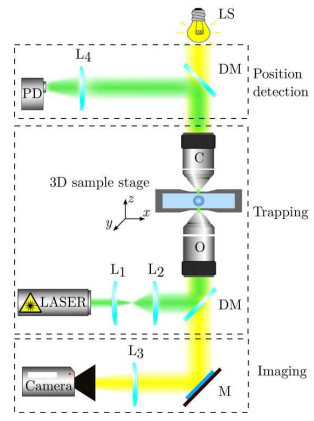
\includegraphics[scale=.85]{OT.PNG}
    \caption{Shown is a relatively simple set up of optical tweezers. There are three main sections of the apparatus highlighted, the section dealing with imaging what is happening in the trap, the actual optical trap itself, and the section housing the position detector. From \textit{Optical tweezers: A comprehensive tutorial from calibration to applications}\cite{ot}}
    \label{fig:OT}
\end{figure}

    A basic example of a single beam optical tweezers set up can be seen in Figure \ref{fig:OT}. Initially, the light exits the laser and passes through a set of lenses that act as a beam widener. After the beam is widened, it is directed to a microscope objective by the use of dichroic aligning mirrors. Dichroic mirrors allow for certain wavelengths of light to pass through them while reflecting others. In the case of optical tweezers, the mirrors can be chosen so that the imagining light required for the camera can pass through the mirrors while the laser light is reflected towards the trap. After the laser is directed to the microscope objective, it passes through and creates the trap\cite{tut}. 
    
    An important quantity associated with the microscope objective is the numerical aperture, which describes the cone of light that exits the objective. To calculate the numerical aperture of an objective, the following equation is used,
    
    \begin{equation}
        NA = nsin(\alpha)
    \end{equation}
    where n represents the refractive index of the medium the light will travel through and $\alpha$ represents the half angular aperture, which is the angle made between the focal point and the axis of the cone\cite{NA}. When a range of numerical apertures are compared, a higher numerical aperture is going to result in a cone of light that is shorter and wider than the cone of light from light passing through a lower numerical aperture. A cone of light that is short and wide is going to do a better job at focusing the light. This is part of the reason optical tweezers set ups more often than not use a high numerical aperture objective as the trap is going to be more effective.
        
    The medium and object chosen must not both only be transparent, but they must also be chosen such that the refractive index of the bead is larger than the refractive index of the medium. Without this, the optical trap will have a reverse effect and force the object out of the laser\cite{ashkin}. When light passes from one medium to another, it refracts. In the situation where the light is passing from a lower refractive index to a higher one, the light slows down. Applying this to a bead suspended in water (with $n_B > n_m$), the light loses momentum as it passes from the water into the bead. Conservation of momentum tells us that this results in a change in momentum in the bead as well. 

    \subsection{\label{sec:level2}Optical Forces}
    
    When an object is placed into an optical trap, there are specific forces acting on the object that cause it to move towards the beam axis and with the light. The same is true for an already trapped object. Certain optical forces are responsible for keeping the object in the trap's state of equilibrium. There are two separate forces at play. The first of which is the scattering force. The scattering of light off of the object creates a force directed in the direction of the light. The expression for the scattering force\cite{brownian} goes as follows,
    
\begin{equation}
\resizebox{.9\hsize}{!}{$ F_{scat} = \sum_{i=1}^{\infty} (\frac{n_m P_i}{c})[1+R_i cos(2\hat{\theta_i}) \\ -\frac{T_i^2 [cos(2\hat{\theta_i}-2\hat{r_i})+R_i cos(2\hat{\theta_i})]}{1+R_i^2 +2R_i cos(2\hat{r_i})}]$}
\label{scat}
\end{equation}    
    where $n_m$ is the refractive index of the medium, $P_i$ is the power of the ray, $R_i$ and $T_i$ are reflection and transmission coefficients, $\hat{\theta_i}$ and $\hat{r_i}$ are the incidence and transmission angles respectively, and c is the speed of light\cite{brownian}. The expression in the summation is the equation for the scattering force from one specific ray of light. Summing over infinity allows for the total scattering force to account for all of the rays of light. The second force is the gradient force. A gradient in the intensity of the light brings about this force. Looking at Figure \ref{fig:forces}, the light rays drop in intensity the farther away one gets from the beam axis. Using this fact, it can be seen that rays closer to the beam axis, such as ray b in the diagram, are going to cause a greater force than a farther away ray, such as ray a. As the bead enters the focal point of an optical tweezers set up, the gradient forces balances out the scattering force resulting in the bead remaining in equilibrium. As the bead is moved from equilibrium, whether by force or Brownian motion, the scattering and gradient forces act as restoring forces. The expression for the gradient force is very similar to the scattering force equation. The gradient force\cite{brownian} is given as,
    
\begin{equation}
\resizebox{.9\hsize}{!}{$F_{grad} = \sum_{i=1}^{\infty} (\frac{n_m P_i}{c})[R_i sin(2\hat{\theta_i})-\frac{T_i^2 [sin(2\hat{\theta_i}-2\hat{r_i})+R_i cos(2\hat{\theta_i})]}{1+R_i^2 +2R_i cos(2\hat{r_i})}]$}
\label{grad}
\end{equation}
    where the variables are defined the same as for the scattering force. Summing the equations for an individual ray, again, allows for the total gradient force to be solved for. For both of these equations, the large bracketed term can be simplified to make these expressions much cleaner. The bracketed terms are defined as trapping efficiencies. These trapping efficiencies account for the efficiency of momentum transfer\cite{brownian}. Just as both force equations were for an individual ray and slightly different, the trapping efficiencies are as well. Each beam of light has a specific scattering and gradient force that separately have their own trapping efficiencies. Performing this simplification to equations \ref{scat} and \ref{grad}, the following equations result,
    
    \begin{equation}
        F_{scat} = \sum_{i=1}^{\infty} (\frac{n_m P_i}{c}) Q_{scat, i}
    \end{equation}
    
    \begin{equation}
        F_{grad} = \sum_{i=1}^{\infty} (\frac{n_m P_i}{c}) Q_{grad, i}
    \end{equation}
    
    A total trapping efficiency for a particular ray of light\cite{brownian} can be found using,
    
    \begin{equation}
    Q_{trap}=\sqrt{Q_{scat}^2 + Q_{grad}^2}
    \end{equation}
    
    
    
\begin{figure}[h]
    \centering
    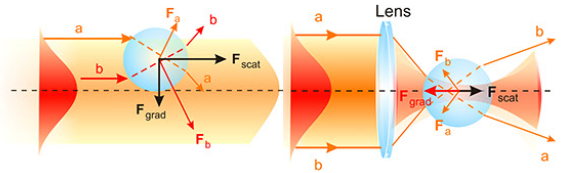
\includegraphics[scale=.57]{Forces diagram.PNG}
    \caption{Shown here is a diagram depicting the optical forces acting on a bead caught in an optical trap. The left most image shows the bead in an unfocused beam, whereas the right most image shows the bead at the focal point of a laser focused through an objective. Gradient and scattering forces are shown. From \textit{Optical Tweezers}\cite{ot}}
    \label{fig:forces}
\end{figure}

    The actual "trap" part of the optical trap is the potential. In the case of optical tweezers, the trapping potential is in the form of a harmonic potential. Harmonic potentials are expressed as,
    
    \begin{equation}
        U(x)=\frac{\kappa}{2}(x-x_eq)^2
    \end{equation}
    where $\kappa_x$ is the trapping stiffness and $x_eq$ is the equilibrium position, the focal point in the case of optical tweezers\cite{brownian}. For harmonic potentials, the restoring force is equal to the displacement of the object. As the object is displaced further and further away from equilibrium, it will be subjected to a larger and larger restoring force. The article \textit{Temperature Effects on Optical Trapping Stability}\cite{brownian} states that, through Boltzmann statistics, the probability density of a particle subject to a harmonic potential is in the form of a Gaussian distribution. Not surprisingly, this implies that we most likely will see the particle found at it's equilibrium point, the focal point. This is exactly what we observe. 


    \subsection{\label{sec:level2}Drawbacks}
    Optical tweezers can bring about a specific set of problems on their own that need to be accounted for and considered when planning on using them for experimentation. Some of these drawbacks that come with using optical tweezers will be reviewed along with some details of what causes them to be an issue. 

        \subsubsection{\label{sec:level3}Brownian Motion}
    Something that must be understood and accounted for to create an optical trap is the Brownian motion of particles. When a particle is placed within a medium, it will undergo interactions with the particles of that medium and motion will result from these collisions\cite{brownian}. As the objects that are being optically trapped are typically on the $\mu m$ scale, they will be subject to this motion. Temperature can be thought of as an expression of how much kinetic energy a system has on average. Each individual particle of that system is going to have it's own kinetic energy that, when changed, has an effect on the temperature. This is also true in the reverse case, as there is an increase in temperature we can expect to see an increase in the kinetic energies of the particles. Looking at an optical tweezers set up. as the laser causes an increase in the temperature of the water around a trapped bead, the kinetic energy of the water molecules are going to become larger and larger. Collisions between the bead and the molecules of water will become more frequent and will result in an increase in random motion. 
    
    For an optical trap to be considered stable, it has to be able to both account for and overcome the effects of Brownian motion. This means that the trap must have a high enough trapping potential for the moving bead to not be able to escape outside the gradient of the laser. In a mathematical sense, this can be expressed as a comparison between two radii. The first of which is the radius of confinement due to Brownian motion in an optical trap after an extended time, $R_p$. This radius can be expressed as $R_p = \sqrt{2 k_b T / \kappa}$. The other radius to consider is the trapping radius, $R_t$. This represents the radius at which an object can be trapped\cite{brownian}. If the bead were to move outside of the trapping radius, then Brownian motion would carry it off, away from the trap. For stability in a trap, the following condition must be met:
    \begin{equation}
        R_t \geq R_p
    \end{equation}
    Upon substituting in the value for $R_p$, this inequality can be solved as such,
    \begin{equation}
        \frac{1}{2} \kappa R_t^2 \geq k_B T
    \end{equation}
    Where $k_B$ is the Boltzmann constant and T is temperature. These quantities represent the trapping potential and the thermal energy respectively\cite{brownian}. Without enough thermal energy for the particle to overcome the potential, the particle will remain trapped. There is a similar issue with the size of the object meant to be trapped. Optical potential forces, that keep the object trapped despite Brownian motion, lower as the object becomes smaller\cite{brownian}. Rather than raising the thermal energy closer to the potential in this case, the potential is lowered to potentially below the thermal energy. Thankfully, if this is considered when choosing an object to be trapped, the issue can be mitigated.


        \subsubsection{\label{sec:level3}Radiation Damage and Localized Heating}
    Due to the use of organic objects, damage to the sample from the laser must be considered. For this reason, higher frequency lasers are avoided. Near infrared lasers are favored due to their lower frequency compared to visible light. The energy of the light is therefore lower than other forms of light and can be found with the equation,
        \begin{equation}
            E = \frac{hc}{\lambda}
        \end{equation}
    where E is the energy of a photon in the laser, h is Planck's Constant, c is the speed of light, and $\lambda$ is the wavelength of the light. If the wavelength of the laser used in Ashkin's initial radiation pressure experiment, 514.5 $nm$, is compared to a near infrared laser (NIR) with relatively low wavelength, 750 $nm$, there is an energy difference of $45.7\%$. NIR lasers typically range from 750-1200 $nm$\cite{NIR}, so it is possible to increase the difference of energies even further resulting in even less radiation damage to a sample. 
    
    Unfortunately, the use of NIR lasers is not a foolproof plan to eliminating damage to organic samples. They bring with them the problem of localized heating. The temperature increase generated from a NIR laser is estimated to be around 10-15 $C$\cite{NIR}. Heat can be an issue for both organic material and optical trapping. Certain properties of the DNA, or any other biopolymer being studied, could be changed in the presence of increased temperature\cite{NIR}. This has the possibility of making data collection difficult in experiments of this nature due to the fact that conclusions cannot be drawn when the DNA is mechanically different than intended. As discussed previously, Brownian motion is known to increase alongside an increase in temperature. The heating from the NIR laser is no exception to this. As the laser heats the medium around the object being trapped, that object will be subjected to increasing Brownian motion.



\section{DNA Stretching}
    Set up for an experiment meant to test the elasticity of DNA will consist of three core parts. The first of which is the optically trapped bead. Analyzing the displacement of the light passing through the bead allows for calculations of the force applied to be done. One of the main benefits to using optical tweezers in experiments like this, outside of the precision, is the ability to find the forces in such a way. Another bead acts as the mode of extension. It is connected by suction to a micropipet, that can be moved to generate the desired extension. Most important is the DNA, which is connected between this set of beads. 
    
    
\begin{figure}[h]
    \centering
    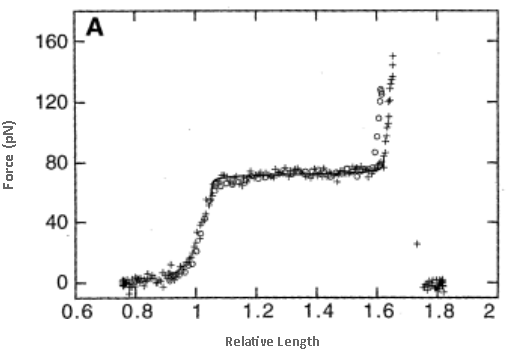
\includegraphics[scale=.64]{DNA extension plot.PNG}
    \caption{Shown here is a plot of the force applied (in pN) versus the relative length of the DNA (with respect to the contour length). From \textit{DNA: An Extensible Molecule}\cite{extensible}}
    \label{fig:DNA Ex}
\end{figure}

    \subsection{\label{sec:level2}Pre-expansion}
    Upon first separating the beads and stretching the B-DNA, very little force is required to increase the length. This hold true until the DNA begins to approach it's contour length. The contour length of DNA is the number of nucleotides present multiplied by the length of those nucleotides. In simpler terms, it is the max length of the DNA laid out flat. To stretch the DNA the first 90\% of it's contour length, only around 3 $pN$ of force is required\cite{extensible}. It is at this point where the force required to extend the DNA further rises rapidly. 




    \subsection{\label{sec:level2}Expansion}
    Little extension will be gained from increased pulling until a force of approximately 65 $pN$ is applied\cite{overstretching}. Once this force is reached, there is a distinct discontinuity in the elasticity of the DNA molecule. An extension to around 1.7 times the contour length can be achieved within only a 2-3 $pN$ range\cite{overstretching}. As mentioned previously, the contour length is determined by taking the number of nucleotides and multiplying it by the length of the nucleotides. Experiments show that the distance per base pair increases during this time, resulting in the increased contour length. Exactly what the mechanism is behind this transition is not entirely known; however it is clear that there is a structural change that takes place at this point that what is observed can be attributed to. 
    
    Looking at Figure \ref{fig:DNA Ex}, it can be seen that around the 65-70 $pN$ range there is a transition where the increased force required for extension levels off quickly. The DNA molecule behaves elastically similar to how it did prior to any extension and increases in length with little force required. If force is removed from the DNA, the extension process is shown to be reversible\cite{NIR}. 

    \subsection{\label{sec:level2}Theories}
    
    The first theory, described in the article \textit{Overstretching b-dna: The elastic
    response of individual double-stranded and single-stranded dna molecules}\cite{overstretching}, proposes that the extension is a result of bonds holding the base pairs together breaking and the DNA unwinding to form a ladder like structure\cite{overstretching}. 

    The second theory states that the extension models the DNA as a chain of base pairs with two separate states, referred to as B-DNA (unstretched) and S-DNA (expanded). Cluzel et al.\cite{extensible} represented the second theory with their analysis. The two separate states have their own associated lengths and energies. Following this theory, it would result that the extension is a result of a conformational transition\cite{extensible}.

\section{Conclusion}
    In review, optical trapping and optical tweezers set ups have been found to be particularly useful across a range of scientific fields. Neuroscientists, physicists, and biologists alike have adopted this technology and used it to expand their research. Use of optical tweezers on B-DNA is a fairly popular application and was the main application focused on in this review. 
    
    There are certain key attributes to optical tweezers that allow the set up to function. Discussed first was the numerical aperture of the microscope objective used to create the trap. Higher numerical aperture values yield a shorter, wider, more focused beam that is ideal for trapping. Depending on the experiment, a lower numerical aperture objective may be used to place the focal point further into the medium. Second came the selection of the refractive indices of the object and medium. A higher refractive index of the bead meant that the light would slow down upon changing mediums, resulting in a changed momentum of the bead. This pulls the bead towards the focal point by means of scattering and gradient forces. Considerations that should be made when choosing the apparatus of an experiment have been discussed to highlight potential complications from using an optical tweezers set up. These considerations included accounting for Brownian motion and laser wavelength choice. 
    
    As the use of optical tweezers to study DNA was the primary focus of this review, experiments performed employing optical tweezers set ups were brought to discussion. Some of the experimental findings and data collected from these experiments along with some analysis is shown in order to understand why this research is being done. Although the exact process that is occurring is unknown, two of the predominant theories offering explanation were brought in as a way to catch a reader up to what researchers are currently considering and speculating.
    



\nocite{*}
\bibliography{Sources}

\end{document}